\section{Probability Assessment and Thresholds}
\subsection{Training-Derived Probability Assessment}
Ranking, calibrated probability, and a binary decision are separate outputs. We assess the raw probabilities of logistic regression, the random forest, and XGBoost on their common random-test population. Reliability diagrams compare average scores with observed cancellation proportions within ten equal-frequency bins; repeated scores can reduce the number of distinct bins. The diagonal is a calibration reference, while departures describe the fixed model on this particular population \citep{sklearncalibration}.

We also evaluate a sigmoid mapping, fitted by univariate logistic regression to the clipped logit of training out-of-fold scores (probabilities clipped to \([10^{-6},1-10^{-6}]\), \(C=10^6\)). For the validation threshold analysis, this mapping is cross-fitted over the existing five OOF folds: each validation fold is mapped using a sigmoid fitted to the other folds' OOF score--label pairs. A final mapping fitted to all training OOF pairs transforms random-test scores. No random-test labels fit the mapping or determine a threshold.

This is a practical post-selection assessment, not fully nested calibration validation. Base OOF models share fitting records, candidate selection has already used these folds, and the OOF score distribution may differ from scores of the model refitted on all training data. Cross-fitting the sigmoid reduces direct reuse of a row's label by its own mapping, but does not remove these dependencies. We do not select a new model using the calibration test results or claim that the mapped probabilities are validated for a future period.

\begin{figure*}[t]
\centering
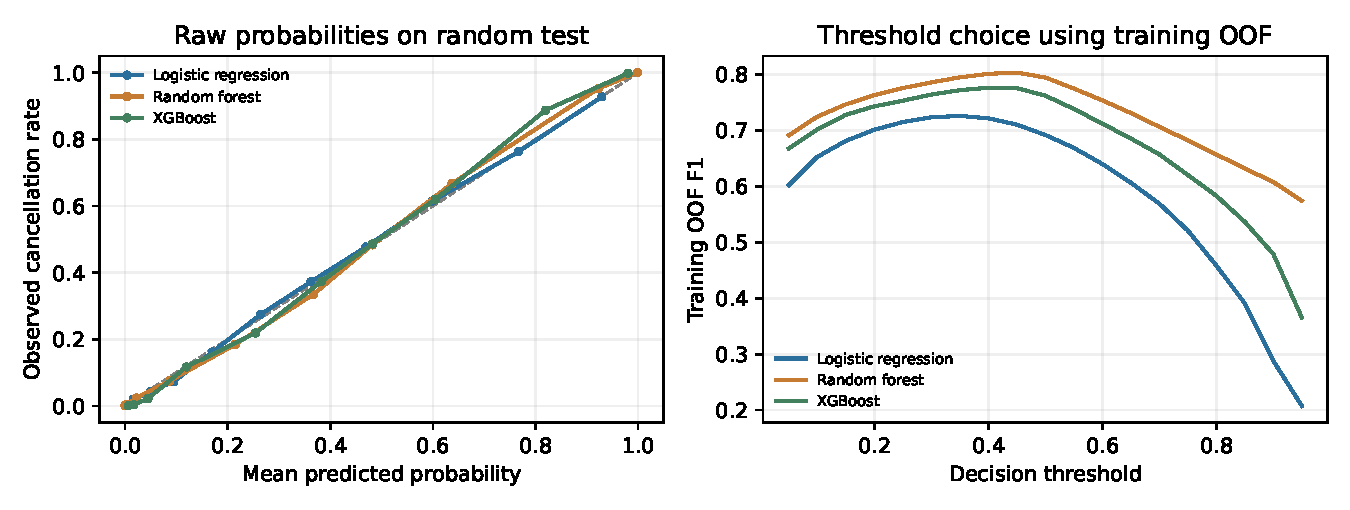
\includegraphics[width=0.98\textwidth]{calibration_and_thresholds.pdf}
\caption{Left: raw-score reliability on random test after all models are fixed. Right: threshold curves from training OOF scores only. Test labels are used to evaluate calibration, not to choose a threshold.}
\label{fig:calibration}
\end{figure*}

At threshold 0.50, sigmoid mapping changes Brier scores from 0.141971 to 0.141964 for logistic regression, 0.097321 to 0.096971 for the forest, and 0.111488 to 0.110991 for XGBoost. Improvements are small; the strongest raw benchmark already has substantially lower Brier error than the linear baseline. Since each fitted mapping is monotone increasing, ROC-AUC and AP remain unchanged in these test outputs. Calibration changes score interpretation and potentially decisions, not the order of bookings in this experiment. Brier scores are independent of the chosen decision threshold.

\subsection{Validation-Selected Thresholds}
For raw and sigmoid scores separately, we search thresholds 0.05--0.95 in increments of 0.05, maximise training OOF F1, and break ties in favour of the smaller threshold. This selects raw thresholds 0.35 for logistic regression, 0.45 for the forest, and 0.40 for XGBoost. We evaluate these already fixed rules on the random test. We do not report a test-optimised threshold or replace the 0.50 baseline results with tuned results in the main comparison.

\begin{table}[t]
\centering
\caption{Random-test decisions at training-selected raw-score thresholds. Thresholds optimise OOF F1, not revenue.}
\label{tab:thresholds}
\begin{tabular}{lrrrr}
\toprule
Model & Threshold & Precision & Recall & F1\\
\midrule
Logistic & 0.35 & 0.657 & 0.814 & 0.727\\
Forest & 0.45 & 0.795 & 0.811 & 0.803\\
XGBoost & 0.40 & 0.720 & 0.838 & 0.775\\
\bottomrule
\end{tabular}
\end{table}

For the forest, changing the threshold from 0.50 to 0.45 raises recall from 0.752 to 0.811 and F1 from 0.795 to 0.803, while precision falls from 0.843 to 0.795. False negatives decrease from 2,191 to 1,666, but false positives increase from 1,240 to 1,854. This creates 525 additional correctly flagged cancellations alongside 614 additional false alarms. Whether that trade-off is worthwhile depends on the review action, staff capacity, and guest contact costs.

The sigmoid models select the same coarse-grid thresholds as their raw counterparts, with test F1 values 0.727, 0.803, and 0.775 respectively after rounding. Their small differences do not justify a claim of a large classification benefit. For the benchmark, we retain the raw forest and report 0.50 as the common comparison threshold, with 0.45 as a separate candidate review rule. Neither threshold is established as optimal for a hotel's economic objective or for the later-arrival population.
